\documentclass{article}

%%\usepackage{fullpage, epic, eepic}
\usepackage{wso}

%% Inicio do documento
\begin{document}

%\addtolength{\voffset}{-4cm}
\textheight=1005pt
% \headsep=10pt
% \oddsidemargin=0pt
% \parskip=6pt

\thispagestyle{empty}

\begin{sidewaysfigure}

%\begin{figure}%
  \centering
  \subfloat[\textbf{Linux$^{\mathbf{Std}}$ - Sem carga} \newline
  \vskip 1mm VM:     8.9, DP:     0.3,  Min:     8.7, Max:    18.4 ]{%
    \label{fig:ker23Sem}%
    {\scalebox{0.8}{\input{fig/ker23Sem}}}} \hspace{4pt}%
  \subfloat[\textbf{Linux$^{\mathbf{Std}}$ - Com carga} \newline
  \vskip 1mm VM:    10.4, DP:     1.9,  Min:     8.8, Max:    67.7]{%
    \label{fig:ker23Tot}%
    {\scalebox{0.8}{% GNUPLOT: LaTeX picture with Postscript
\begingroup
  \makeatletter
  \providecommand\color[2][]{%
    \GenericError{(gnuplot) \space\space\space\@spaces}{%
      Package color not loaded in conjunction with
      terminal option `colourtext'%
    }{See the gnuplot documentation for explanation.%
    }{Either use 'blacktext' in gnuplot or load the package
      color.sty in LaTeX.}%
    \renewcommand\color[2][]{}%
  }%
  \providecommand\includegraphics[2][]{%
    \GenericError{(gnuplot) \space\space\space\@spaces}{%
      Package graphicx or graphics not loaded%
    }{See the gnuplot documentation for explanation.%
    }{The gnuplot epslatex terminal needs graphicx.sty or graphics.sty.}%
    \renewcommand\includegraphics[2][]{}%
  }%
  \providecommand\rotatebox[2]{#2}%
  \@ifundefined{ifGPcolor}{%
    \newif\ifGPcolor
    \GPcolorfalse
  }{}%
  \@ifundefined{ifGPblacktext}{%
    \newif\ifGPblacktext
    \GPblacktextfalse
  }{}%
  % define a \g@addto@macro without @ in the name:
  \let\gplgaddtomacro\g@addto@macro
  % define empty templates for all commands taking text:
  \gdef\gplbacktext{}%
  \gdef\gplfronttext{}%
  \makeatother
  \ifGPblacktext
    % no textcolor at all
    \def\colorrgb#1{}%
    \def\colorgray#1{}%
  \else
    % gray or color?
    \ifGPcolor
      \def\colorrgb#1{\color[rgb]{#1}}%
      \def\colorgray#1{\color[gray]{#1}}%
      \expandafter\def\csname LTw\endcsname{\color{white}}%
      \expandafter\def\csname LTb\endcsname{\color{black}}%
      \expandafter\def\csname LTa\endcsname{\color{black}}%
      \expandafter\def\csname LT0\endcsname{\color[rgb]{1,0,0}}%
      \expandafter\def\csname LT1\endcsname{\color[rgb]{0,1,0}}%
      \expandafter\def\csname LT2\endcsname{\color[rgb]{0,0,1}}%
      \expandafter\def\csname LT3\endcsname{\color[rgb]{1,0,1}}%
      \expandafter\def\csname LT4\endcsname{\color[rgb]{0,1,1}}%
      \expandafter\def\csname LT5\endcsname{\color[rgb]{1,1,0}}%
      \expandafter\def\csname LT6\endcsname{\color[rgb]{0,0,0}}%
      \expandafter\def\csname LT7\endcsname{\color[rgb]{1,0.3,0}}%
      \expandafter\def\csname LT8\endcsname{\color[rgb]{0.5,0.5,0.5}}%
    \else
      % gray
      \def\colorrgb#1{\color{black}}%
      \def\colorgray#1{\color[gray]{#1}}%
      \expandafter\def\csname LTw\endcsname{\color{white}}%
      \expandafter\def\csname LTb\endcsname{\color{black}}%
      \expandafter\def\csname LTa\endcsname{\color{black}}%
      \expandafter\def\csname LT0\endcsname{\color{black}}%
      \expandafter\def\csname LT1\endcsname{\color{black}}%
      \expandafter\def\csname LT2\endcsname{\color{black}}%
      \expandafter\def\csname LT3\endcsname{\color{black}}%
      \expandafter\def\csname LT4\endcsname{\color{black}}%
      \expandafter\def\csname LT5\endcsname{\color{black}}%
      \expandafter\def\csname LT6\endcsname{\color{black}}%
      \expandafter\def\csname LT7\endcsname{\color{black}}%
      \expandafter\def\csname LT8\endcsname{\color{black}}%
    \fi
  \fi
  \setlength{\unitlength}{0.0500bp}%
  \begin{picture}(7200.00,5040.00)%
    \gplgaddtomacro\gplbacktext{%
      \csname LTb\endcsname%
      \put(1034,594){\makebox(0,0)[r]{\strut{}$0.0$}}%
      \put(1034,1117){\makebox(0,0)[r]{\strut{}$5.0$}}%
      \put(1034,1640){\makebox(0,0)[r]{\strut{}$10.0$}}%
      \put(1034,2162){\makebox(0,0)[r]{\strut{}$15.0$}}%
      \put(1034,2685){\makebox(0,0)[r]{\strut{}$20.0$}}%
      \put(1034,3208){\makebox(0,0)[r]{\strut{}$25.0$}}%
      \put(1034,3731){\makebox(0,0)[r]{\strut{}$30.0$}}%
      \put(1034,4253){\makebox(0,0)[r]{\strut{}$35.0$}}%
      \put(1034,4776){\makebox(0,0)[r]{\strut{}$40.0$}}%
      \put(1166,374){\makebox(0,0){\strut{}$ 0$}}%
      \put(2109,374){\makebox(0,0){\strut{}$ 10$}}%
      \put(3053,374){\makebox(0,0){\strut{}$ 20$}}%
      \put(3996,374){\makebox(0,0){\strut{}$ 30$}}%
      \put(4939,374){\makebox(0,0){\strut{}$ 40$}}%
      \put(5883,374){\makebox(0,0){\strut{}$ 50$}}%
      \put(6826,374){\makebox(0,0){\strut{}$ 60$}}%
      \put(396,2685){\rotatebox{90}{\makebox(0,0){\strut{}Lat\^encia em $\mu s$}}}%
      \put(3996,110){\makebox(0,0){\strut{}Tempo de observa\c{c}\~ao em $s$}}%
    }%
    \gplgaddtomacro\gplfronttext{%
    }%
    \gplbacktext
    \put(0,0){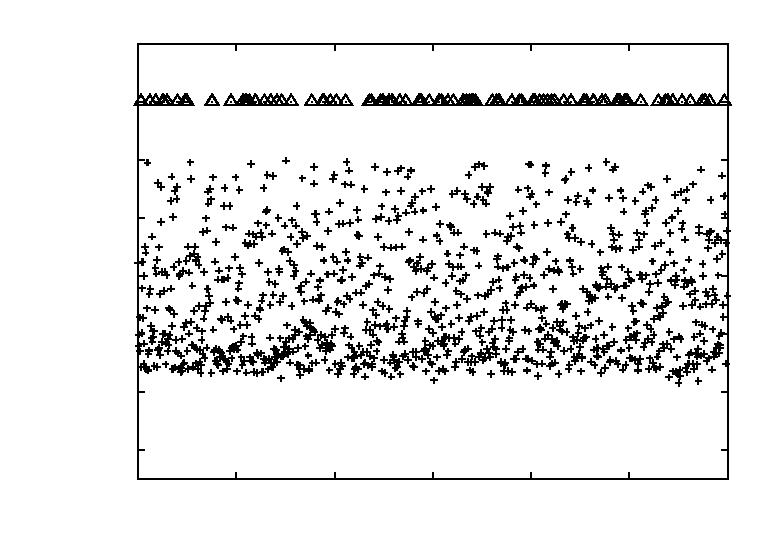
\includegraphics{fig/ker23Tot}}%
    \gplfronttext
  \end{picture}%
\endgroup
}}} \hspace{4pt}%
\end{sidewaysfigure}

%   \caption[Lat�ncias de interrup��o]{Lat�ncia de interrup��o com
%     freq��ncia de escrita na PP de $20 Hz$.}
%   \label{fig:latIrq}%
%\end{figure}

\end{document}


\begin{figure}%
  \centering
  \subfloat[\textbf{Linux$^{\mathbf{Std}}$ - Sem carga} \newline
  \vskip 1mm VM:     8.9, DP:     0.3,  Min:     8.7, Max:    18.4 ]{%
    \label{fig:ker23Sem}%
    {\scalebox{0.58}{\input{fig/ker23Sem}}}} \hspace{4pt}%
  \subfloat[\textbf{Linux$^{\mathbf{Std}}$ - Com carga} \newline
  \vskip 1mm VM:    10.4, DP:     1.9,  Min:     8.8, Max:    67.7]{%
    \label{fig:ker23Tot}%
    {\scalebox{0.58}{% GNUPLOT: LaTeX picture with Postscript
\begingroup
  \makeatletter
  \providecommand\color[2][]{%
    \GenericError{(gnuplot) \space\space\space\@spaces}{%
      Package color not loaded in conjunction with
      terminal option `colourtext'%
    }{See the gnuplot documentation for explanation.%
    }{Either use 'blacktext' in gnuplot or load the package
      color.sty in LaTeX.}%
    \renewcommand\color[2][]{}%
  }%
  \providecommand\includegraphics[2][]{%
    \GenericError{(gnuplot) \space\space\space\@spaces}{%
      Package graphicx or graphics not loaded%
    }{See the gnuplot documentation for explanation.%
    }{The gnuplot epslatex terminal needs graphicx.sty or graphics.sty.}%
    \renewcommand\includegraphics[2][]{}%
  }%
  \providecommand\rotatebox[2]{#2}%
  \@ifundefined{ifGPcolor}{%
    \newif\ifGPcolor
    \GPcolorfalse
  }{}%
  \@ifundefined{ifGPblacktext}{%
    \newif\ifGPblacktext
    \GPblacktextfalse
  }{}%
  % define a \g@addto@macro without @ in the name:
  \let\gplgaddtomacro\g@addto@macro
  % define empty templates for all commands taking text:
  \gdef\gplbacktext{}%
  \gdef\gplfronttext{}%
  \makeatother
  \ifGPblacktext
    % no textcolor at all
    \def\colorrgb#1{}%
    \def\colorgray#1{}%
  \else
    % gray or color?
    \ifGPcolor
      \def\colorrgb#1{\color[rgb]{#1}}%
      \def\colorgray#1{\color[gray]{#1}}%
      \expandafter\def\csname LTw\endcsname{\color{white}}%
      \expandafter\def\csname LTb\endcsname{\color{black}}%
      \expandafter\def\csname LTa\endcsname{\color{black}}%
      \expandafter\def\csname LT0\endcsname{\color[rgb]{1,0,0}}%
      \expandafter\def\csname LT1\endcsname{\color[rgb]{0,1,0}}%
      \expandafter\def\csname LT2\endcsname{\color[rgb]{0,0,1}}%
      \expandafter\def\csname LT3\endcsname{\color[rgb]{1,0,1}}%
      \expandafter\def\csname LT4\endcsname{\color[rgb]{0,1,1}}%
      \expandafter\def\csname LT5\endcsname{\color[rgb]{1,1,0}}%
      \expandafter\def\csname LT6\endcsname{\color[rgb]{0,0,0}}%
      \expandafter\def\csname LT7\endcsname{\color[rgb]{1,0.3,0}}%
      \expandafter\def\csname LT8\endcsname{\color[rgb]{0.5,0.5,0.5}}%
    \else
      % gray
      \def\colorrgb#1{\color{black}}%
      \def\colorgray#1{\color[gray]{#1}}%
      \expandafter\def\csname LTw\endcsname{\color{white}}%
      \expandafter\def\csname LTb\endcsname{\color{black}}%
      \expandafter\def\csname LTa\endcsname{\color{black}}%
      \expandafter\def\csname LT0\endcsname{\color{black}}%
      \expandafter\def\csname LT1\endcsname{\color{black}}%
      \expandafter\def\csname LT2\endcsname{\color{black}}%
      \expandafter\def\csname LT3\endcsname{\color{black}}%
      \expandafter\def\csname LT4\endcsname{\color{black}}%
      \expandafter\def\csname LT5\endcsname{\color{black}}%
      \expandafter\def\csname LT6\endcsname{\color{black}}%
      \expandafter\def\csname LT7\endcsname{\color{black}}%
      \expandafter\def\csname LT8\endcsname{\color{black}}%
    \fi
  \fi
  \setlength{\unitlength}{0.0500bp}%
  \begin{picture}(7200.00,5040.00)%
    \gplgaddtomacro\gplbacktext{%
      \csname LTb\endcsname%
      \put(1034,594){\makebox(0,0)[r]{\strut{}$0.0$}}%
      \put(1034,1117){\makebox(0,0)[r]{\strut{}$5.0$}}%
      \put(1034,1640){\makebox(0,0)[r]{\strut{}$10.0$}}%
      \put(1034,2162){\makebox(0,0)[r]{\strut{}$15.0$}}%
      \put(1034,2685){\makebox(0,0)[r]{\strut{}$20.0$}}%
      \put(1034,3208){\makebox(0,0)[r]{\strut{}$25.0$}}%
      \put(1034,3731){\makebox(0,0)[r]{\strut{}$30.0$}}%
      \put(1034,4253){\makebox(0,0)[r]{\strut{}$35.0$}}%
      \put(1034,4776){\makebox(0,0)[r]{\strut{}$40.0$}}%
      \put(1166,374){\makebox(0,0){\strut{}$ 0$}}%
      \put(2109,374){\makebox(0,0){\strut{}$ 10$}}%
      \put(3053,374){\makebox(0,0){\strut{}$ 20$}}%
      \put(3996,374){\makebox(0,0){\strut{}$ 30$}}%
      \put(4939,374){\makebox(0,0){\strut{}$ 40$}}%
      \put(5883,374){\makebox(0,0){\strut{}$ 50$}}%
      \put(6826,374){\makebox(0,0){\strut{}$ 60$}}%
      \put(396,2685){\rotatebox{90}{\makebox(0,0){\strut{}Lat\^encia em $\mu s$}}}%
      \put(3996,110){\makebox(0,0){\strut{}Tempo de observa\c{c}\~ao em $s$}}%
    }%
    \gplgaddtomacro\gplfronttext{%
    }%
    \gplbacktext
    \put(0,0){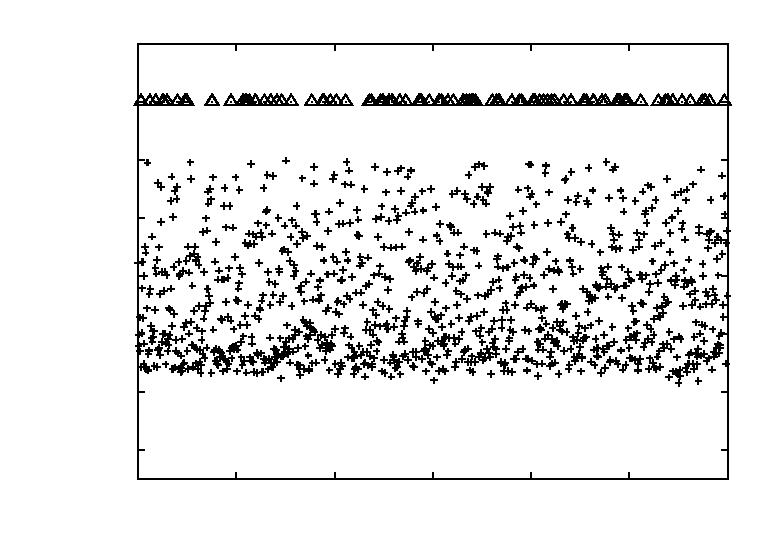
\includegraphics{fig/ker23Tot}}%
    \gplfronttext
  \end{picture}%
\endgroup
}}} \hspace{4pt}%

  \vspace{7pt}%
  \subfloat[\textbf{Linux$^{\mathbf{Prt}}$ - Sem carga} \newline
  \vskip 1mm VM: 21.5, DP: 1.7, Min: 20.3, Max: 45.1]{%
    \label{fig:preSem}%
    {\scalebox{0.58}{\input{fig/preSem}}}} \hspace{4pt}%
  \subfloat[\textbf{Linux$^{\mathbf{Prt}}$ - Com carga} \newline
  \vskip 1mm VM: 58.5, DP: 26.4, Min: 17.2, Max: 245.9]{%
    \label{fig:preTot}%
    {\scalebox{0.58}{\input{fig/preTot}}}} \hspace{4pt}%

  \vspace{7pt}%
  \subfloat[\textbf{Linux$^{\mathbf{Xen}}$ - Sem carga} \newline
  \vskip 1mm VM: 9.0, DP: 0.1, Min: 8.8, Max: 11.1]{%
    \label{fig:xenSem}%
    {\scalebox{0.58}{\input{fig/xenSem}}}} \hspace{4pt}%
  \subfloat[\textbf{Linux$^{\mathbf{Xen}}$ - Com carga} \newline
  \vskip 1mm VM: 10.2, DP: 0.1, Min: 8.8, Max: 20.8]{%
    \label{fig:xenTot}%
    {\scalebox{0.58}{\input{fig/xenTot}}}} \hspace{4pt}%

  \caption[Lat�ncias de interrup��o]{Lat�ncia de interrup��o com
    freq��ncia de escrita na PP de $20 Hz$.}
  \label{fig:latIrq}%
\end{figure}


\begin{sidewaysfigure}
%\begin{figure}%
  \centering
  \subfloat[\textbf{Linux$^{\mathbf{Std}}$ - Sem carga} \newline
  \vskip 1mm {\footnotesize VM:     8.9, DP:     0.3,  Min:     8.7, Max:    18.4 }]{%
    \label{fig:ker23Sem}%
    {\scalebox{0.42}{\input{fig/ker23Sem}}}} \hspace{4pt}%
  %\vspace{7pt}%
  \subfloat[\textbf{Linux$^{\mathbf{Prt}}$ - Sem carga} \newline
  \vskip 1mm {\footnotesize VM: 21.5, DP: 1.7, Min: 20.3, Max: 45.1}]{%
    \label{fig:preSem}%
    {\scalebox{0.42}{\input{fig/preSem}}}} \hspace{4pt}%
  %\vspace{7pt}%
  \subfloat[\textbf{Linux$^{\mathbf{Rtai}}$ - Sem carga} \newline
  \vskip 1mm {\footnotesize VM: 8.7, DP: 0.1, Min: 8.8, Max: 10.7}]{%
    \label{fig:xenSem}%
    {\scalebox{0.42}{\input{fig/rtaiSem}}}} \hspace{4pt}%
  %\vspace{7pt}%
  \subfloat[\textbf{Linux$^{\mathbf{Xen}}$ - Sem carga} \newline
  \vskip 1mm {\footnotesize VM: 9.0, DP: 0.1, Min: 8.8, Max: 11.1}]{%
    \label{fig:xenSem}%
    {\scalebox{0.42}{\input{fig/xenSem}}}} \hspace{4pt}%

  \subfloat[\textbf{Linux$^{\mathbf{Std}}$ - Com carga} \newline
  \vskip 1mm {\footnotesize VM:    10.4, DP:     1.9,  Min:     8.8, Max:    67.7}]{%
    \label{fig:ker23Tot}%
    {\scalebox{0.4}{% GNUPLOT: LaTeX picture with Postscript
\begingroup
  \makeatletter
  \providecommand\color[2][]{%
    \GenericError{(gnuplot) \space\space\space\@spaces}{%
      Package color not loaded in conjunction with
      terminal option `colourtext'%
    }{See the gnuplot documentation for explanation.%
    }{Either use 'blacktext' in gnuplot or load the package
      color.sty in LaTeX.}%
    \renewcommand\color[2][]{}%
  }%
  \providecommand\includegraphics[2][]{%
    \GenericError{(gnuplot) \space\space\space\@spaces}{%
      Package graphicx or graphics not loaded%
    }{See the gnuplot documentation for explanation.%
    }{The gnuplot epslatex terminal needs graphicx.sty or graphics.sty.}%
    \renewcommand\includegraphics[2][]{}%
  }%
  \providecommand\rotatebox[2]{#2}%
  \@ifundefined{ifGPcolor}{%
    \newif\ifGPcolor
    \GPcolorfalse
  }{}%
  \@ifundefined{ifGPblacktext}{%
    \newif\ifGPblacktext
    \GPblacktextfalse
  }{}%
  % define a \g@addto@macro without @ in the name:
  \let\gplgaddtomacro\g@addto@macro
  % define empty templates for all commands taking text:
  \gdef\gplbacktext{}%
  \gdef\gplfronttext{}%
  \makeatother
  \ifGPblacktext
    % no textcolor at all
    \def\colorrgb#1{}%
    \def\colorgray#1{}%
  \else
    % gray or color?
    \ifGPcolor
      \def\colorrgb#1{\color[rgb]{#1}}%
      \def\colorgray#1{\color[gray]{#1}}%
      \expandafter\def\csname LTw\endcsname{\color{white}}%
      \expandafter\def\csname LTb\endcsname{\color{black}}%
      \expandafter\def\csname LTa\endcsname{\color{black}}%
      \expandafter\def\csname LT0\endcsname{\color[rgb]{1,0,0}}%
      \expandafter\def\csname LT1\endcsname{\color[rgb]{0,1,0}}%
      \expandafter\def\csname LT2\endcsname{\color[rgb]{0,0,1}}%
      \expandafter\def\csname LT3\endcsname{\color[rgb]{1,0,1}}%
      \expandafter\def\csname LT4\endcsname{\color[rgb]{0,1,1}}%
      \expandafter\def\csname LT5\endcsname{\color[rgb]{1,1,0}}%
      \expandafter\def\csname LT6\endcsname{\color[rgb]{0,0,0}}%
      \expandafter\def\csname LT7\endcsname{\color[rgb]{1,0.3,0}}%
      \expandafter\def\csname LT8\endcsname{\color[rgb]{0.5,0.5,0.5}}%
    \else
      % gray
      \def\colorrgb#1{\color{black}}%
      \def\colorgray#1{\color[gray]{#1}}%
      \expandafter\def\csname LTw\endcsname{\color{white}}%
      \expandafter\def\csname LTb\endcsname{\color{black}}%
      \expandafter\def\csname LTa\endcsname{\color{black}}%
      \expandafter\def\csname LT0\endcsname{\color{black}}%
      \expandafter\def\csname LT1\endcsname{\color{black}}%
      \expandafter\def\csname LT2\endcsname{\color{black}}%
      \expandafter\def\csname LT3\endcsname{\color{black}}%
      \expandafter\def\csname LT4\endcsname{\color{black}}%
      \expandafter\def\csname LT5\endcsname{\color{black}}%
      \expandafter\def\csname LT6\endcsname{\color{black}}%
      \expandafter\def\csname LT7\endcsname{\color{black}}%
      \expandafter\def\csname LT8\endcsname{\color{black}}%
    \fi
  \fi
  \setlength{\unitlength}{0.0500bp}%
  \begin{picture}(7200.00,5040.00)%
    \gplgaddtomacro\gplbacktext{%
      \csname LTb\endcsname%
      \put(1034,594){\makebox(0,0)[r]{\strut{}$0.0$}}%
      \put(1034,1117){\makebox(0,0)[r]{\strut{}$5.0$}}%
      \put(1034,1640){\makebox(0,0)[r]{\strut{}$10.0$}}%
      \put(1034,2162){\makebox(0,0)[r]{\strut{}$15.0$}}%
      \put(1034,2685){\makebox(0,0)[r]{\strut{}$20.0$}}%
      \put(1034,3208){\makebox(0,0)[r]{\strut{}$25.0$}}%
      \put(1034,3731){\makebox(0,0)[r]{\strut{}$30.0$}}%
      \put(1034,4253){\makebox(0,0)[r]{\strut{}$35.0$}}%
      \put(1034,4776){\makebox(0,0)[r]{\strut{}$40.0$}}%
      \put(1166,374){\makebox(0,0){\strut{}$ 0$}}%
      \put(2109,374){\makebox(0,0){\strut{}$ 10$}}%
      \put(3053,374){\makebox(0,0){\strut{}$ 20$}}%
      \put(3996,374){\makebox(0,0){\strut{}$ 30$}}%
      \put(4939,374){\makebox(0,0){\strut{}$ 40$}}%
      \put(5883,374){\makebox(0,0){\strut{}$ 50$}}%
      \put(6826,374){\makebox(0,0){\strut{}$ 60$}}%
      \put(396,2685){\rotatebox{90}{\makebox(0,0){\strut{}Lat\^encia em $\mu s$}}}%
      \put(3996,110){\makebox(0,0){\strut{}Tempo de observa\c{c}\~ao em $s$}}%
    }%
    \gplgaddtomacro\gplfronttext{%
    }%
    \gplbacktext
    \put(0,0){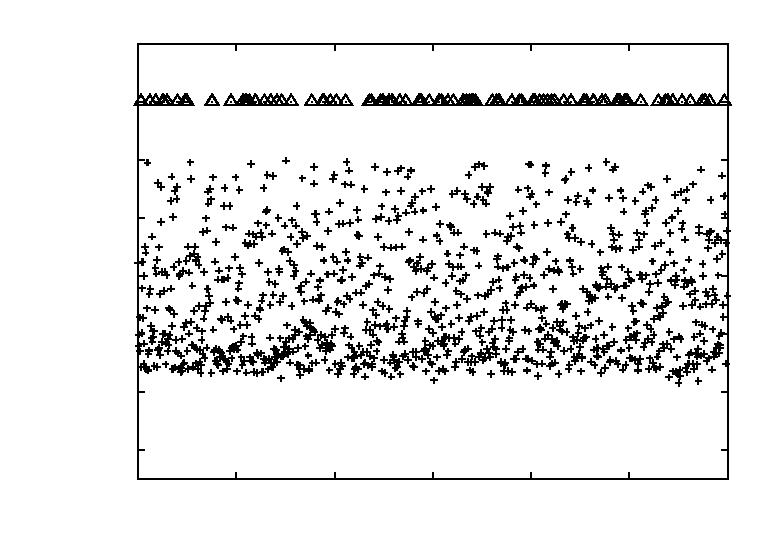
\includegraphics{fig/ker23Tot}}%
    \gplfronttext
  \end{picture}%
\endgroup
}}} \hspace{4pt}%
  \subfloat[\textbf{Linux$^{\mathbf{Prt}}$ - Com carga} \newline
  \vskip 1mm {\footnotesize VM: 58.5, DP: 26.4, Min: 17.2, Max: 245.9}]{%
    \label{fig:preTot}%
    {\scalebox{0.4}{\input{fig/preTot}}}} \hspace{4pt}%
  \subfloat[\textbf{Linux$^{\mathbf{Rtai}}$ - Com carga} \newline
  \vskip 1mm {\footnotesize VM: 10.0, DP: 0.8, Min: 8.8, Max: 20.8}]{%
    \label{fig:xenTot}%
    {\scalebox{0.4}{\input{fig/rtaiTot}}}} \hspace{4pt}%
  \subfloat[\textbf{Linux$^{\mathbf{Xen}}$ - Com carga} \newline
  \vskip 1mm {\footnotesize VM: 10.4, DP: 0.7, Min: 8.9, Max: 20.8}]{%
    \label{fig:xenTot}%
    {\scalebox{0.4}{\input{fig/xenTot}}}} \hspace{4pt}%

  \caption[Lat�ncias de interrup��o]{Lat�ncia de interrup��o com
    freq��ncia de escrita na PP de $20 Hz$.}
  \label{fig:latIrq}%
\end{sidewaysfigure}
%\end{figure}
